\documentclass{standalone}

\usepackage{tikz}
\usetikzlibrary{intersections,decorations.markings}

\begin{document}
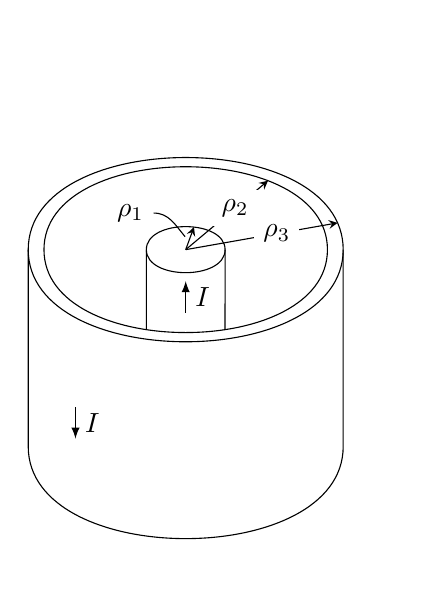
\begin{tikzpicture}
%\draw[thick,gray] (-3,-4) grid (3,3);
%\draw[thin,gray,step=0.2] (-3,-4) grid (3,3);
%
%round heads
\draw[name path=k1] (-0.5,0) to [out=-90,in=-90] (0.5,0) to [out=90,in=90] (-0.5,0);
\draw[name path=k2] (-1.8,0) to [out=-90,in=-90] (1.8,0)  to [out=90,in=90] (-1.8,0);
\draw[name path=k3] (-2,0) to [out=-90,in=-90] (2,0)  to [out=90,in=90] (-2,0);
%outer vertical section
\draw(2,0) --++(0,-2.5) to [out=-90,in=-90] (-2,-2.5)--++(0,2.5);
%inner vertical edges
\path[name path=k4] (-0.5,0) --++(0,-2);
\path[name path=k5] (0.5,0) --++(0,-2);
\draw[name intersections={of=k2 and k4}](-0.5,0)--(intersection-1);
\draw[name intersections={of=k2 and k5}](0.5,0)--(intersection-1);
%radii
\path[name path=k6] (0,0) --++(70:3);
\path[name path=k7] (0,0) --++(40:3);
\path[name path=k8] (0,0) --++(10:3);
\draw[-stealth,name intersections={of=k6 and k1}](0,0)--(intersection-1)coordinate[pos=0.4](innerMost);
\draw[-stealth,name intersections={of=k7 and k2}](0,0)--(intersection-1)node[pos=0.6,fill=white]{$\rho_2$};
\draw[-stealth,name intersections={of=k8 and k3}](0,0)--(intersection-1)node[pos=0.6,fill=white]{$\rho_3$};
\draw[] (innerMost)++(-0.05,0.05) to [out=130,in=0]++(-0.4,0.3)node[left]{$\rho_1$};
%currents
\draw[latex-](0,-0.4)--++(0,-0.4)node[pos=0.5,right]{$I$};
\draw[-latex](-1.4,-2)--++(0,-0.4)node[pos=0.5,right]{$I$};
\end{tikzpicture}
\end{document} 
